\section{Evietania Charis Sujadi 1174051}
\subsection{Penjelasan Shapefile dengan PySHP}
Shapefile adalah format data untuk menyimpan data spasial non topologi yang berbasis vektor. sedangkan pyshp adalah sebuah library yang digunakan untuk dapat menjalankan shapefile \hfill\break

\subsection{Berikut tahapan membuat shapefile dengan pyshp}
\begin{enumerate}
	\item No 1
	\lstinputlisting{src/1174051/2/1.py}
	\begin{figure}[H]
		
\includegraphics[width=6cm]{figures/1174051/2/1.PNG}
		\centering
		\caption{Hasil No 1}
	\end{figure}
	\item Nomor 2
	\lstinputlisting{src/1174051/2/2.py}
	\begin{figure}[H]
		
\includegraphics[width=6cm]{figures/1174051/2/2.PNG}
		\centering
		\caption{Hasil No 2}
	\end{figure}
	\item Nomor 3
	\lstinputlisting{src/1174051/2/3.py}
	\begin{figure}[H]
		
\includegraphics[width=6cm]{figures/1174051/2/3.PNG}
		\centering
		\caption{Hasil No 3}
	\end{figure}
	\item Nomor 4
	\lstinputlisting{src/1174051/2/4.py}
	\begin{figure}[H]
        
\includegraphics[width=6cm]{figures/1174051/2/4.PNG}
		\centering
		\caption{Hasil No 4}
	\end{figure}
	\item Nomor 5
	\lstinputlisting{src/1174051/2/5.py}
	\begin{figure}[H]
        
\includegraphics[width=6cm]{figures/1174051/2/5.PNG}
		\centering
		\caption{Hasil No 5}
	\end{figure}
	\item Nomor 6
	\lstinputlisting{src/1174051/2/6.py}
	\begin{figure}[H]
        
\includegraphics[width=6cm]{figures/1174051/2/6.PNG}
		\centering
		\caption{Hasil No 6}
	\end{figure}
	\item Nomor 7
	\lstinputlisting{src/1174051/2/7.py}
	\begin{figure}[H]
        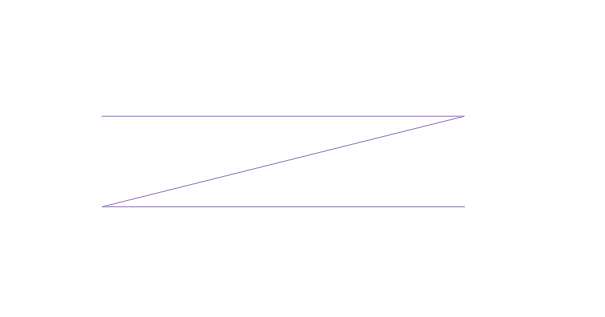
\includegraphics[width=6cm]{figures/1174051/2/7.PNG}
		\centering
		\caption{Hasil No 7}
	\end{figure}
	\item Nomor 8
	\lstinputlisting{src/1174051/2/8.py}
	\begin{figure}[H]
        
\includegraphics[width=6cm]{figures/1174051/2/8.PNG}
		\centering
		\caption{Hasil No 8}
	\end{figure}
	\item Nomor 9
	\lstinputlisting{src/1174051/2/9.py}
	\begin{figure}[H]
		
\includegraphics[width=6cm]{figures/1174051/2/9.PNG}
		\centering
		\caption{Hasil No 9}
	\end{figure}
	\item Nomor 10
	\lstinputlisting{src/1174051/2/10.py}
	\begin{figure}[H]
        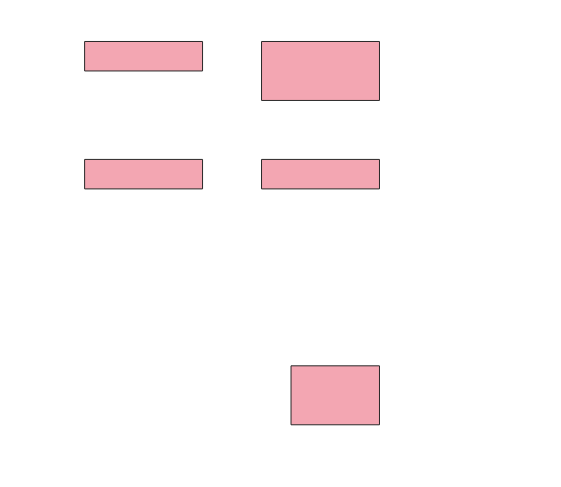
\includegraphics[width=6cm]{figures/1174051/2/10.PNG}
		\centering
		\caption{Hasil No 10, NPM saya adalah 1174051, hasil modulus 8 dari NPM 1174051 adalah 3, jadi membuat bidang persegi panjang dan angka kedua terakhir di NPM saya adalah 5 maka saya akan membuat 5 buah persegi panjang}
	\end{figure}
\end{enumerate}
\subsection{Link}
 \href{https://www.youtube.com/watch?v=RE9UUjy9_00}{Video Youtube}
\subsection{Plagiarism}
\begin{figure}[H]
	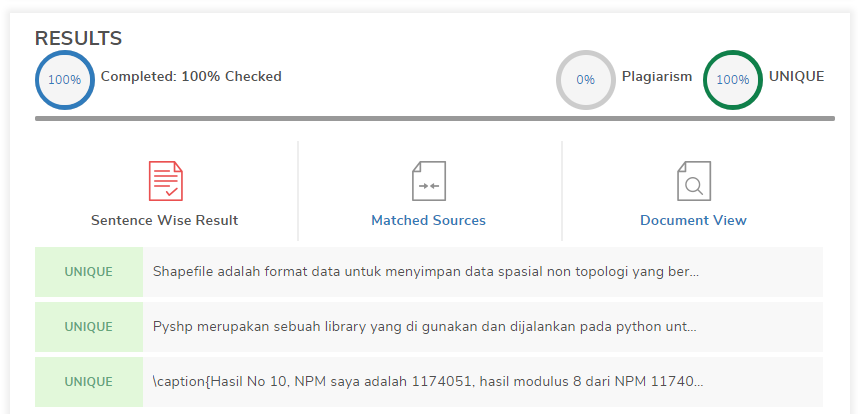
\includegraphics[width=4cm]{figures/1174051/2/plagiat.png}
	\centering
	\caption{Plagiarism}
\end{figure}